\documentclass[a4paper,12pt]{article}
\usepackage[a4paper,top=1.3cm,bottom=2cm,left=1.5cm,right=1.5cm,marginparwidth=0.75cm]{geometry}
%%% Работа с русским языком
\usepackage{cmap}					% поиск в PDF
\usepackage{mathtext} 				% русские буквы в фомулах
\usepackage[T2A]{fontenc}			% кодировка
\usepackage[utf8]{inputenc}			% кодировка исходного текста
\usepackage[english,russian]{babel}	% локализация и переносы

\usepackage{graphicx}
\usepackage{mathtools}
\usepackage{wrapfig}
\usepackage{tabularx}
\usepackage{amssymb}
\usepackage{hyperref}
\usepackage[rgb]{xcolor}
\hypersetup{colorlinks=true,urlcolor=blue}
\setcounter{secnumdepth}{0}
%% Шрифты
\usepackage{euscript}	 % Шрифт Евклид
\usepackage{amsmath}
\usepackage{mathtools}
%%% Заголовок
\author{Tsvetkova Amelia}
\title{Лабораторная работа по общей физике}

\date{\today}
\begin{document}
\begin{titlepage}
    \newpage
    \begin{center}
    {\large МОСКОВСКИЙ ФИЗИКО-ТЕХНИЧЕСКИЙ ИНСТИТУТ (НАЦИОНАЛЬНЫЙ ИССЛЕДОВАТЕЛЬСКИЙ УНИВЕРСИТЕТ)}
    \vspace{1cm}

    {\largeФизтех-школа аэрокосмических технологий}
    \vspace{6em}
    \end{center}
    
    \vspace{1.2em}

    \begin{center}
    \Large Лабораторная работа №5.8.1 \\
    Тепловое излучение
    \linebreak
    \end{center}
    
    \vspace{11em}
    
    \begin{flushright}
                       {\large Работу выполнила\\
                       Цветкова Амелия Антоновна\\
                       Б03-305 }
    \end{flushright}

    \vspace{\fill}

    \begin{center}
    Долгопрудный, 2025
    \end{center}

    \end{titlepage}

\section{Цели работы}
\begin{enumerate}
    \item При помощи модели абсолютно черного тела (АЧТ) провести измерения температуры оптическим пирометром с исчезающей нитью и термопарой;
    \item Исследовать излучение накаленных тел с различной испускательной способностью;
    \item Определить постоянные Планка и Стефана–Больцмана.
\end{enumerate}

\section{Теоретические сведения}

Для измерения температуры разогретых тел, удаленных от наблюдателя, применяют методы оптической пирометрии, основанные на использовании зависимости испускательной способности исследуемого тела от температуры. Различают три температуры, функционально связанные с истинной термодинамической температурой и излучательной способностью тела: радиационную $T_{\text{рад}}$, цветовую $T_{\text{цв}}$ и яркостную $T_{\text{ярк}}$.

Под \texttt{радиационной (энергетической)} температурой понимают температуру абсолютно черного тела, при которой его интегральная испускательная способность одинакова с интегральной испускательной способностью исследуемого тела.

Под \texttt{цветовой} температурой исследуемого тела понимают температуру абсолютно черного тела, при которой отношение их спектральных испускательных способностей для двух заданных длин волн одинаково.

Под \texttt{яркостной} температурой понимают температуру абсолютно черного тела, при которой его спектральная испускательная способность равна спектральной испускательной способности исследуемого тела при той же длине волны. Именно эту температуру мы будем измерять в данной работе.

Измерение яркостной температуры раскаленного тела производится при помощи оптического пирометра с исчезающей нитью, основанного на визуальном сравнении яркости раскаленной нити с яркостью изображения исследуемого тела. Равенство видимых яркостей, наблюдаемых через монохроматический светофильтр ($\lambda = 6500$ Å), фиксируется по исчезновению изображения нити на фоне раскаленного тела. Яркостный метод измерения температуры основан, в соответствии с формулой Планка, на зависимости испускательной способности абсолютно черного тела от температуры и длины волны.

Оптический пирометр представляет собой зрительную трубу, внутри которой имеется накаливаемая нить, расположенная в плоскости изображения исследуемого раскаленного тела, а также темно-красный светофильтр ($\lambda = 6500$ Å). Через окуляр одновременно наблюдается изображение исследуемого тела и раскаленной нити.

Если в том узком спектральном интервале, который пропускается светофильтром, яркость нити меньше яркости раскаленного тела, то нить видится темной полоской на светлом фоне, и наоборот. При совпадении яркостей нить перестает быть видимой на фоне изображения раскаленного тела. Регулировка яркости нити осуществляется изменением тока, протекающего через нее.

Пирометр с исчезающей нитью включает в себя объектив, окуляр, монохроматический (красный) светофильтр, позволяющий рассматривать в лучах красного цвета (6500 Å) нить пирометра на фоне изображения накаленного исследуемого тела. Пирометр имеет два диапазона измерений: $700 \div 1200^\circ$C и $1200 \div 2000^\circ$C. Переключение осуществляется введением серого светофильтра, регулировка накала нити пирометра выведена на лицевую панель блока питания.

Модель АЧТ представляет собой керамическую трубку диаметром 3 мм и длиной 50 мм, закрытую с одного конца и окруженную для теплоизоляции внешним кожухом. Нагрев трубки осуществляется намотанной на ней нихромовой спиралью, питаемой от источника тока. Полость трубки и особенно ее дно излучают практически как абсолютно черное тело. Температура модели АЧТ измеряется хромель-алюмелевой термопарой, один спай которой вмонтирован в дно трубки, а другой находится при комнатной температуре на клемме цифрового вольтметра В7-38, измеряющего ЭДС термопары.

В работе исследуются три образца. Один образец выполнен в виде керамической трубки с набором колец из различных материалов, нагреваемой изнутри нихромовой спиралью. Материалы колец имеют различную испускательную способность. Спираль подключается к источнику питания с помощью переключателя и может нагревать трубку до температуры около $1100^\circ$C. Термодинамическая температура колец практически одинакова и равна температуре трубки.

Другой исследуемый образец — вольфрамовая нить электрической лампочки. Она питается от источника, когда переключатель находится в соответствующем положении. Сила тока через вольфрамовую нить измеряется с помощью прибора В7-22А. Падение напряжения на самой нити измеряется непосредственно вольтметром В7-22А. Таким образом, зная показания обоих приборов, можно определить мощность, потребляемую нитью лампочки.

Источник питания, используемый в работе, снабжен устройством, отключающим в случае перегрузки прибор от потребителя, в этот момент загорается сигнальная лампочка «перегрузка» на передней панели прибора.

Вначале с помощью модели абсолютно черного тела проверяется правильность работы пирометра, а затем с его помощью исследуется излучение различных материалов и вольфрамовой нити накаливания. Необходимая для обработки проводимых в данной работе измерений зависимость между яркостной и термодинамической температурами вольфрама приведена на рис.:

\begin{figure}[h]
\centering
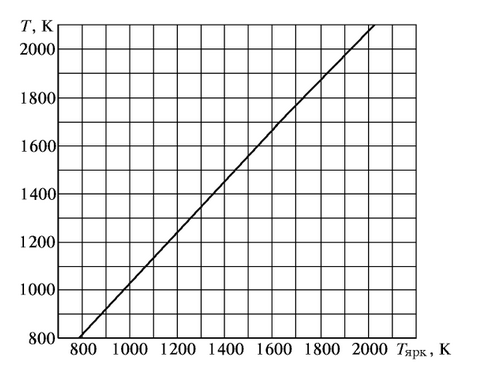
\includegraphics[width=0.6\textwidth]{img1.png}
\caption{График зависимости $T = f(T_{\text{ярк}})$ для вольфрама}
\label{img1}
\end{figure}

По результатам измерений мощности излучения вольфрамовой нити можно судить о справедливости закона Стефана–Больцмана. Для этого следует мощность, потребляемую нитью, приравнять к излучаемому ею за единицу времени количеству энергии. Если бы нить излучала как абсолютно черное тело, то баланс потребляемой и излучаемой энергии определялся бы соотношением:
$$
W = \sigma S (T^4 - T_0^4),
$$
где $W$ — потребляемая нитью электрическая мощность, $S$ — площадь излучающей поверхности нити, $T$ — температура нити, $T_0$ — температура окружающей среды.

Однако вольфрамовая нить излучает как нечерное тело. Среди нечерных тел выделяются так называемые серые тела, для которых характер распределения излучения совершенно подобен спектру абсолютно черного тела, но излучение ослаблено по сравнению с ним в $\varepsilon_T$ раз для любой длины волны при данной температуре тела $T$.

Если предположить, что нить излучает как серое тело, то выражение можно записать в виде:
$$
W = \varepsilon_T S \sigma T^4,
$$
где мы учли, что реально температура вольфрама намного выше температуры окружающей среды.

\begin{figure}[h]
\centering
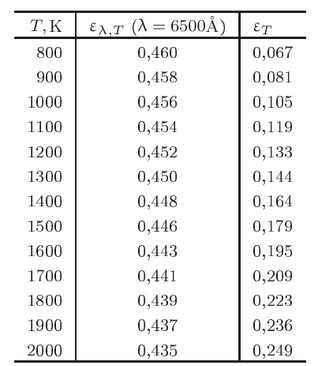
\includegraphics[width=0.4\textwidth]{img4.png}
\caption{Поправочные коэффициенты излучения для вольфрама}
\label{tab1}
\end{figure}

Измерив температуру вольфрамовой нити в зависимости от подводимой мощности, можно убедиться в справедливости закона Стефана–Больцмана применительно к серому телу (в данном случае к вольфраму). Для этого нужно построить график зависимости $W(T)$ в логарифмическом масштабе и по наклону определить показатель степени $n$ исследуемой температурной зависимости. Понятно, что в пределах погрешности показатель степени должен быть близок к четырем.

\begin{figure}[h]
\centering
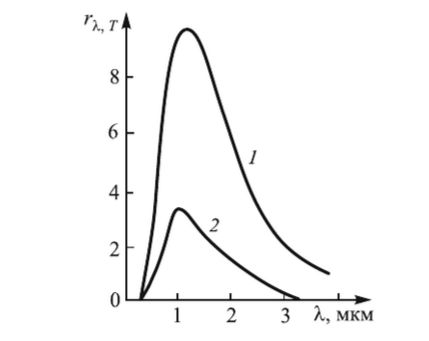
\includegraphics[width=0.4\textwidth]{img2.png}
\caption{Распределение энергии в спектре излучения: 1 - абсолютно черное тело; 2 - вольфрам. Температура 2450 К}
\end{figure}

Из формулы можно определить также и величину постоянной $\sigma$ в законе Стефана–Больцмана. Некоторое отличие величин $n$ и $\sigma$, полученных экспериментально, от теоретических значений может быть объяснено особенностью вольфрама, у которого наблюдается селективность излучения в коротковолновом диапазоне. Селективность излучения вольфрама становится особенно заметной при ярком накале, когда его температура составляет около 2400 K. Оказывается, что излучение в видимой области спектра существенно больше, чем это следует из распределения Планка, примененного к серому телу.

В частности, именно поэтому вольфрам и выбран в качестве материала в лампах накаливания. При меньших температурах селективность излучения проявляется слабее, но при этом все большую роль играет теплоотвод от нити, что в свою очередь ведет к ошибке в определении величин $n$ и $\sigma$.

Проведя измерения в диапазоне температур от 800 до $1500^\circ$C, можно выяснить, в каком участке этого интервала температур вольфрамовая нить лампы накаливания излучает почти как серое тело, т.е. величины $n$ и $\sigma$ соответствуют теоретическим значениям.

\section{Экспериментальная установка}

Экспериментальная установка состоит из оптического пирометра 9, модели абсолютно черного тела (АЧТ), трех исследуемых образцов (18, 19, 20), блока питания (1) и цифровых вольтметров В7-22А и В7-38.

Пирометр 9 с исчезающей нитью включает в себя объектив 10, окуляр 8, монохроматический (красный) светофильтр 4, позволяющий рассматривать в лучах красного цвета (6500 Å) нить пирометра на фоне изображения накаленного исследуемого тела. Перемещение светофильтра осуществляется сектором 12. Пирометр имеет два диапазона измерений: 700 ÷ 1200°C и 1200 ÷ 2000°C. Переключение осуществляется введением серого светофильтра при помощи переключателя 11 «Включение». Регулировка накала нити пирометра выведена на лицевую панель блока питания.

\begin{figure}[h]
\centering
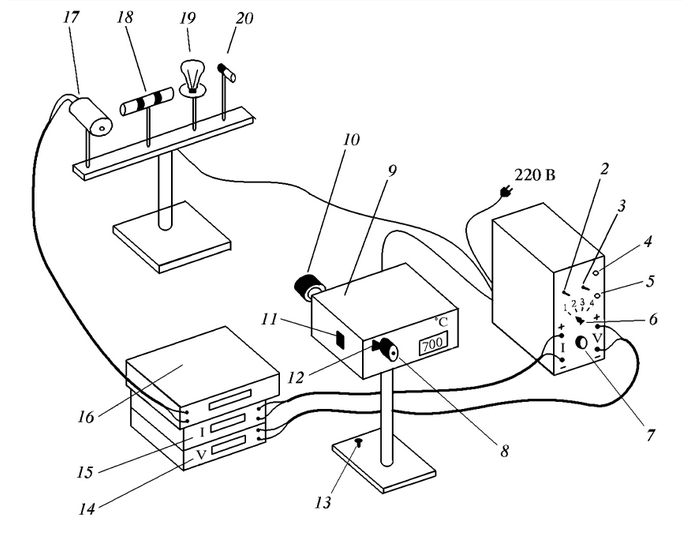
\includegraphics[width=0.6\textwidth]{img3.png}
\caption{Схема экспериментальной установки: 1 — блок питания; 2 — тумблер включения питания пирометра и образцов; 3 — тумблер нагрева нити пирометра: «Быстро» — вверх, «Медленно» — вниз; 4 — кнопка «Нагрев нити»; 5 — кнопка «Охлаждение нити»; 6 — тумблер переключения образцов; 7 — регулятор мощности нагрева образцов; 8 — окуляр пирометра; 9 — корпус пирометра; 10 — объектив пирометра; 11 — переключение диапазонов: 700–1200°С — вниз, 1200–2000°С — вверх; 12 — ручка перемещения красного светофильтра; 13 — регулировочный винт; 14 — вольтметр (напряжение на лампе накаливания); 15 — амперметр (ток через образцы); 16 — вольтметр в цепи термопары; 17 — модель АЧТ; 18 — трубка с кольцами из материалов с разной излучательной способностью; 19 — лампа накаливания; 20 — неоновая лампочка.}
\end{figure}

Модель АЧТ представляет собой керамическую трубку диаметром 3 мм и длиной 50 мм, закрытую с одного конца и окруженную для теплоизоляции внешним кожухом. Нагрев трубки осуществляется намотанной на ней нихромовой спиралью, питаемой от источника тока. Полость трубки и особенно ее дно излучают практически как абсолютно черное тело. Температура модели АЧТ измеряется хромель-алюмелевой термопарой, один спай которой вмонтирован в дно трубки, а другой находится при комнатной температуре на клемме цифрового вольтметра В7-38, измеряющего ЭДС термопары.

В работе исследуются три образца. Один образец выполнен в виде керамической трубки с набором колен из различных материалов, нагреваемой изнутри нихромовой спиралью. Материалы колен имеют различную испускательную способность. Спираль подключается к источнику питания 1 с помощью переключателя 6 (положение 2) и может нагревать трубку до температуры около 1100°С. Термодинамическая температура колен практически одинакова и равна температуре трубки.

Другой исследуемый образец — вольфрамовая нить электрической лампочки. Она питается от источника 1, когда переключатель 6 находится в положении 3. Сила тока через вольфрамовую нить измеряется с помощью прибора В7-22А (15). Падение напряжения на самой нити измеряется непосредственно вольтметром В7-22А (16). Таким образом, зная показания обоих приборов, можно определить мощность, потребляемую нитью лампочки.

Источник питания 1, используемый в работе, снабжен устройством, отключающим в случае перегрузки прибор от потребителя, в этот момент загорается сигнальная лампочка «перегрузка» на передней панели прибора. Если это произойдет, то надо отключить питание прибора от сети 220 В и уменьшить напряжение на его выходе, а затем повторно включить источник питания.

\section{Ход работы}
\subsection{I. Изучение работы оптического пирометра}
\begin{enumerate}
    \item Выводим оба светофильтра пирометра с помощью переключателей;
    \item Подключаем питание и доводим показания пирометра до 900-950$^\circ C$. Добиваемся четкого изображения поверхности дна модели АЧТ;
    \item Определим по шкале пирометра значение яркостной температуры модели АЧТ. Одновременно измеряем температуру модели АЧТ с помощью хромель-алюмелевой термопары и цифрового вольтметра. Постоянная термопары 41 мкВ/$^\circ$C.

    \begin{table}[h!]
    \centering
    \begin{tabular}{||c||c|c|c||}
    \hline
    Температура яркостная АЧТ, $^\circ C$ & 944 & 973 & 962 \\
    \hline
    Напряжение на термопаре, В & 38.96 & 39.17 & 39.06 \\
    \hline
    Температура на пирометре, $^\circ C$ & 970 & 975.4 & 973 \\
    \hline
    Разность значений, $\%$ & 2.8 & 0.2 & 1.14 \\
    \hline
    \end{tabular}
    \end{table}

    Убедились, что значения температуры, получаемые обоими способами, мало отличаются друг от друга (не более 3$\%$).
\end{enumerate}

\subsection{II. Измерение яркостной температуры накаленных тел}

Этот эксперимент показывает, что различные тела, нагретые до одинаковой термодинамической температуры, имеют различную яркостную температуру.

\begin{enumerate}

    \item Направим пирометр на поверзность керамиической трубки с кольцами из различных материалов;
    \item Измерим яркостную температуру поверхности трубки и каждого из колец:

    \begin{table}[h!]
    \centering
    \begin{tabular}{||c||c|c|c||}
    \hline
    Температура яркостная АЧТ, $^\circ C$ & 813 &  & 837 \\
    \hline
    Температура левого кольца, $^\circ$C & 830 & 825 & 829 \\
    \hline 
    Температура правого кольца, $^\circ$C & 805 & 799 & 803 \\
    \hline
    \end{tabular}
    \end{table}

Несовпадение яркостной температуры у различных тел, нагретых до одинаковой термодинамической температуры, вытекает из того, что эти две величины связаны, в том числе, через спектральный коэффициент поглощения, который зависит ото материала. 
    
\end{enumerate}


\subsection{III. Проверка закона Стефана-Больцмана}

\begin{enumerate}
    \item Направляем пирометр на нить лампы накаливания. Постепенно увеличивая накал нити лампы, измеряем пирометром яркостную температуру нити;
    \item Для каждого значения измеренной яркостной температуры находим термодинамическую, пользуясь графиком $T=f_1(T_\text{ярк})$. Вычисляем для каждой термодинамической температуры мощность, потребляемую нитью лампы.

    Из рисунка \ref{img1}: $T_{\text{терм}} = 1.04 \cdot T_{\text{ярк}} - 32$
    
    \begin{table}[h!]
    \centering
    \begin{tabular}{||c|c|c|c|c||}
    \hline
    $I$, мА & $U$, В & $T_{\text{ярк}}$, $^\circ$C & $T_{\text{терм}}$, $^\circ$C & $W=IU$, мВт \\
    \hline
    \hline
    0.493 & 1.516 & 908 & 912.3 & 747.4 \\
    0.489 & 1.487 & 999 & 1007.0 & 727.1 \\
    0.556 & 2.054 & 1100 & 1112.0 & 1142.0 \\
    0.616 & 2.612 & 1200 & 1216.0 & 1609.0 \\
    0.723 & 3.685 & 1300 & 1320.0 & 2663.0 \\
    0.894 & 5.671 & 1400 & 1424.0 & 5070.0 \\
    1.015 & 7.222 & 1500 & 1528.0 & 7330.0 \\
    1.128 & 8.830 & 1600 & 1632.0 & 9960.0 \\
    1.127 & 8.800 & 1700 & 1736.0 & 9917.6 \\
    \hline
    \end{tabular}
    \end{table}
    $$
    \sigma_{T_{\text{терм}}} = 1.04 \cdot \sigma_{T_{\text{ярк}}} = 1.04 \cdot 2.0 = 2.1^\circ \text{C}
    $$

    $$
    \sigma_W = W \cdot \sqrt{\left(\frac{\sigma_I}{I}\right)^2 + \left(\frac{\sigma_U}{U}\right)^2}\quad \Longleftrightarrow \quad \sigma_W = \sqrt{(U \cdot \sigma_I)^2 + (I \cdot \sigma_U)^2}
    $$

    \begin{table}[h!]
    \centering
    \begin{tabular}{||c|c|c|c|c||}
    \hline
    $\sigma_I$, мА & $\sigma_U$, В & $\sigma_{T_{\text{ярк}}}$, $^\circ$C & $\sigma_{T_{\text{терм}}}$, $^\circ$C & $\sigma_W$, мВт \\
    \hline
    \hline
    0.003 & 0.005 & 2 & 2.1 & 5.2 \\
    0.003 & 0.005 & 2 & 2.1 & 5.1 \\
    0.003 & 0.005 & 2 & 2.1 & 6.9 \\
    0.003 & 0.005 & 2 & 2.1 & 8.7 \\
    0.003 & 0.005 & 2 & 2.1 & 12.8 \\
    0.003 & 0.005 & 2 & 2.1 & 19.4 \\
    0.003 & 0.005 & 2 & 2.1 & 26.3 \\
    0.003 & 0.005 & 2 & 2.1 & 32.9 \\
    0.003 & 0.005 & 2 & 2.1 & 32.8 \\
    \hline
    \end{tabular}
    \end{table}
    
    \item Для проверки закона Стефана-Больцмана построим в логарифмическом масштабе график зависимости $W = \varepsilon_TBT^n$, т.е. функцию
    $$
    \ln{W} = \ln{(\varepsilon_TB)} + n\ln{T}
    $$
    и определим величину $n$ как тангенс угла наклона прямой в области высоких температур, когда мощность, подводимая к нити, практически полностью расходуется на излучение.

    \begin{figure}[h]
    \centering
    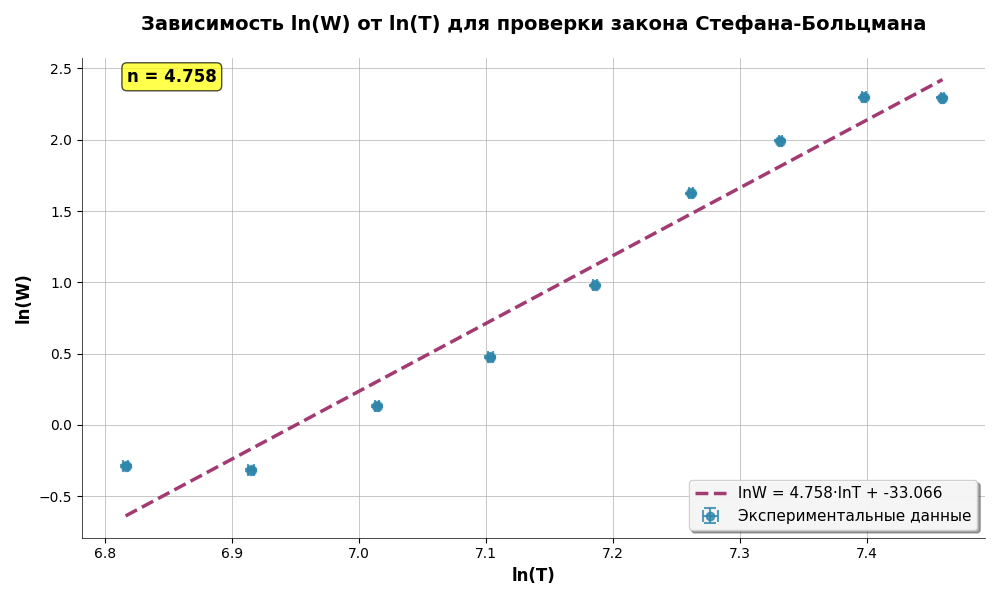
\includegraphics[width=0.9\textwidth]{graph1.png}
    \end{figure}

    Погрешности коэффициентов(т.к. погрешности точек малы):
    $$
    \sigma_k = \sqrt{\frac{n}{n \sum (\ln T_i)^2 - (\sum \ln T_i)^2} \cdot \frac{\sum [\ln W_i - (k \ln T_i + b)]^2}{n-2}}=0.042
    $$
    $$
    \sigma_b = \sqrt{\frac{\sum (\ln T_i)^2}{n \sum (\ln T_i)^2 - (\sum \ln T_i)^2} \cdot \frac{\sum [\ln W_i - (k \ln T_i + b)]^2}{n-2}}=0.350
    $$

    \begin{center}
        \boxed{n=4.758\pm0.042(\varepsilon=0.88\%)}
    \end{center}

    Значение $\varepsilon_T$ берется из рисунка \ref{tab1}. Известно, что $B = S \cdot \varepsilon_T$, где $S$ - эффективная площадь излучающей поверхности нити лампы при температуре более 1500$^\circ$C, когда вся нить одинаково накалена; $\sigma$ - постоянная Стефана-Больцмана, $S=0,36\text{см}^2$.

    \item Найдем величину постоянной Стефана-Больцмана по формуле:
    $$
    \sigma = \frac{W}{\varepsilon_T S T^4}
    $$
    для каждого измеренного значения $T$, превышающего 1500К.

    \begin{table}[h!]
    \centering
    \begin{tabular}{||c|c|c|c|c||}
    \hline
    $T$, K & $\varepsilon_T$ & $W$, мВт & $\sigma$, Вт$/$(м$^2\cdot$К$^4$) & $h$, Дж$\cdot$с\\
    \hline
    1500 & 0.179 & 7330.0 & $5.89 \cdot 10^{-8}$ & $6.87 \cdot 10^{-34}$ \\
    \hline
    1600 & 0.195 & 9960.0 & $5.21 \cdot 10^{-8}$ & $7.12 \cdot 10^{-34}$ \\
    \hline
    1700 & 0.209 & 9917.6 & $4.07 \cdot 10^{-8}$ & $7.68 \cdot 10^{-34}$ \\
    \hline
    \end{tabular}
    \end{table}

    \item По найденным значениям $\sigma$ определим величину постоянной Планка по формуле (результаты в таблице выше):
    $$
    h=\sqrt[3]{\frac{2\pi^5k_\text{Б}^4}{15c^2\sigma}}
    $$

    Табличные значения: 
    $$
    \sigma_\text{табл} = 5.670\cdot 10^{-8} \text{Вт}/(\text{м}^2\cdot\text{К}^4) \quad \quad h_\text{табл} = 6.626\cdot 10^{-34} \text{Дж}\cdot \text{с}
    $$
    
    Расчет погрешностей:

    \begin{table}[h!]
    \centering
    \begin{tabular}{||c|c|c|c|c|c||}
    \hline
    $T$, K & $\sigma$, Вт/(м$^2\cdot$К$^4$) & $\delta\sigma$, Вт/(м$^2\cdot$К$^4$) & $\delta\sigma/\sigma$, \% & $\delta h$, Дж$\cdot$с & $\delta h/h$, \% \\
    \hline
    1500 & $5.89 \cdot 10^{-8}$ & $0.89 \cdot 10^{-8}$ & 15.1 & $0.35 \cdot 10^{-34}$ & 5.0 \\
    1600 & $5.21 \cdot 10^{-8}$ & $0.78 \cdot 10^{-8}$ & 15.0 & $0.36 \cdot 10^{-34}$ & 5.1 \\
    1700 & $4.07 \cdot 10^{-8}$ & $0.61 \cdot 10^{-8}$ & 15.0 & $0.38 \cdot 10^{-34}$ & 5.0 \\
    \hline
    \end{tabular}
    \end{table}
    
    $$
    \delta\sigma = \sigma \cdot \sqrt{\left(\frac{\delta W}{W}\right)^2 + \left(\frac{\delta\varepsilon_T}{\varepsilon_T}\right)^2 + \left(4\frac{\delta T}{T}\right)^2}
    $$
    $$
    \delta h = \frac{1}{3}h \cdot \frac{\delta\sigma}{\sigma}
    $$

    
\end{enumerate}

\subsection{IV. Измерение "яркостной температуры" неоновой лампочки}

Направляем пирометр на неоновую лампочку. Дотронувшись до лампочки рукой, убедимся, что термодиннамическая температура лампочки не соотвествует измеренной яркостной.

Яркостная температура: 900 $^\circ$C.

Термодинамическая температура: 30-40 $^\circ$C.

Различие между яркостной и термодинамической температурой неоновой лампочки объясняется тем, что её свечение имеет нетепловую природу. Неон светится из-за электролюминесценции — процесса, при котором атомы неона возбуждаются электрическим полем и испускают кванты света при возвращении в основное состояние. Это излучение имеет узкий спектр (доминирует красная линия ~640 нм) и не подчиняется закону Планка для теплового излучения. Пирометр, откалиброванный на тепловые источники, интерпретирует интенсивность этого монохроматического излучения как высокую температуру, хотя реальная термодинамическая температура лампочки остаётся низкой.

\section{Выводы}
В ходе работы были успешно проведены измерения температур различных тел оптическим пирометром. Показано, что для абсолютно черного тела яркостная и термодинамическая температуры совпадают в пределах погрешности (<3\%), что подтверждает корректность методики измерений. Для тел с различной излучательной способностью (керамические кольца) при одинаковой термодинамической температуре были получены разные яркостные температуры, что демонстрирует зависимость яркостной температуры от материала.

Исследование вольфрамовой нити лампы накаливания подтвердило справедливость закона Стефана-Больцмана для серого тела. Экспериментально полученное значение показателя степени n = 4.758 ± 0.042 хорошо согласуется с теоретическим $n=4$. По измеренным данным были рассчитаны постоянная Стефана-Больцмана ($\sigma \approx 5\cdot10^{-8}$ Вт$/$(м$^2\cdot$К$^4$)) и постоянная Планка ($h \approx 7\cdot10^{-34} $Дж$\cdot$с), которые близки к табличным значениям.

Эксперимент с неоновой лампой наглядно продемонстрировал принципиальное различие между тепловым излучением и нетепловым, при котором яркостная температура не соответствует термодинамической.


\end{document}
